%
% This is the LaTeX template file for lecture notes for CS294-8,
% Computational Biology for Computer Scientists.  When preparing
% LaTeX notes for this class, please use this template.
%
% To familiarize yourself with this template, the body contains
% some examples of its use.  Look them over.  Then you can
% run LaTeX on this file.  After you have LaTeXed this file then
% you can look over the result either by printing it out with
% dvips or using xdvi.
%
% This template is based on the template for Prof. Sinclair's CS 270.

\documentclass[11pt]{article}
\usepackage{charter}
\usepackage{graphicx}
\usepackage{url}
\usepackage{hyperref}
\usepackage{amsmath,amsthm,amssymb}
\usepackage{enumitem}

\setlength{\oddsidemargin}{0 in}
\setlength{\evensidemargin}{0 in}
\setlength{\topmargin}{-0.6 in}
\setlength{\textwidth}{6.5 in}
\setlength{\textheight}{8.5 in}
\setlength{\headsep}{0.75 in}
\setlength{\parindent}{0 in}
\setlength{\parskip}{0.1 in}

\newcommand{\PP}{\mathbb{P}}

%
% The following commands set up the lecnum (lecture number)
% counter and make various numbering schemes work relative
% to the lecture number.
%
\newcounter{lecnum}
\renewcommand{\thepage}{\thelecnum-\arabic{page}}
\renewcommand{\thesection}{\thelecnum.\arabic{section}}
\renewcommand{\theequation}{\thelecnum.\arabic{equation}}
\renewcommand{\thefigure}{\thelecnum.\arabic{figure}}
\renewcommand{\thetable}{\thelecnum.\arabic{table}}

%
% The following macro is used to generate the header.
%
\newcommand{\lecture}[5]{
   \pagestyle{myheadings}
   \thispagestyle{plain}
   \newpage
   \setcounter{lecnum}{#5}
   \setcounter{page}{1}
   \noindent
   \begin{center}
   \framebox{
      \vbox{\vspace{2mm}
    \hbox to 6.28in { {\bf Masters Bridge Program
                        \hfill Summer 2021} }
       \vspace{4mm}
       \hbox to 6.28in { {\Large \hfill Session {#1}: #2  \hfill} }
       \vspace{2mm}
       \hbox to 6.28in { {\it Instructor: #3 \hfill Contact: #4} }
      \vspace{2mm}}
   }
   \end{center}
   \markboth{Session #1: #2}{Session #1: #2}
   \vspace*{4mm}
}


%Use this command for a figure; it puts a figure in wherever you want it.
%usage: \fig{NUMBER}{SPACE-IN-INCHES}{CAPTION}
\newcommand{\fig}[3]{
			\vspace{#2}
			\begin{center}
			Figure \thelecnum.#1:~#3
			\end{center}
	}
% Use these for theorems, lemmas, proofs, etc.
\newtheorem{theorem}{Theorem}[lecnum]
\newtheorem{lemma}[theorem]{Lemma}
\newtheorem{fact}[theorem]{Fact}
\newtheorem{proposition}[theorem]{Proposition}
\newtheorem{claim}[theorem]{Claim}
\newtheorem{corollary}[theorem]{Corollary}
\theoremstyle{definition}
\newtheorem{definition}[theorem]{Definition}
\newtheorem{remark}[theorem]{Remark}
\newtheorem{example}[theorem]{Example}
\newtheorem{exercise}[]{Exercise}
\newenvironment{proofof}[1]{{\em Proof of #1.}}{\hfill%\rule{2mm}{2mm}
\qed}

% **** IF YOU WANT TO DEFINE ADDITIONAL MACROS FOR YOURSELF, PUT THEM HERE:
\renewcommand{\P}{\mathbb{P}}
\newcommand{\Z}{\mathbb{Z}}
\newcommand{\N}{\mathbb{N}}
\renewcommand{\H}{\mathcal{H}}
\renewcommand{\S}{\mathcal{S}}
\newcommand{\C}{\mathbb{C}}
\newcommand{\MAP}{\mathrm{MAP}}
\newcommand{\z}{\mathbf{z}}
\newcommand{\e}{\mathbf{e}}
\newcommand{\w}{\mathbf{w}}
\newcommand{\x}{\mathbf{x}}
\newcommand{\Rp}{\mathbb{R}_{>0}}
\newcommand{\im}{\mathrm{Im}}
\newcommand{\sign}{\mathrm{sign}}
\newcommand{\E}{\mathbb{E}}
\newcommand{\FF}{\mathcal{F}}
\newcommand{\R}{\mathbb{R}}
\newcommand{\lbr}{\langle}
\newcommand{\rbr}{\rangle}
\newcommand{\indi}{\mathds{1}}

\newcommand{\xmin}{X_{\text{min}}}
\newcommand{\xmax}{X_{\text{max}}}
\newcommand{\cov}{\text{Cov}}
\newcommand{\corr}{\text{Corr}}
\newcommand{\var}{\text{Var}}

\begin{document}
\lecture{6}{Dependence between random variables}{Bryan Liu}{runjing\_liu@berkeley.edu}{6}

{\bf Supplemental reading: } Pitman, \textit{Probability}
 Chapter 6.

\section{Conditional densities}
Recall that for a discrete random variable $X$,
the conditional distribution of $Y$ given $X = x$ is
\begin{align*}
  \P(Y = y | X = x) = \frac{\P(Y = y, X = x)}{\P(X = x)}.
\end{align*}
However, if $X$ is a continuous random variable, then
the denominator $X = x$ has probability 0,
which results in an undefined expression.

In order to define conditional distributions for
continuous random variables $X$ and $Y$,
we express the conditional distribution in terms of densities.

\fbox{\begin{minipage}{\textwidth}
\textbf{Conditional density of $Y$ given $X = x$}.
For random variables $X$ and $Y$ with joint density $f(x,y)$, for each $x$ with marginal density $f_X(x)>0$,
the conditional density of $Y$ given $X = x$ is the
probability density function
\begin{align}
  f_Y(y | X = x) = \frac{f(x,y)}{f_X(x)}.
  \label{eq:cond_density}
\end{align}
Then for any set $B$,
\begin{align*}
  \P(g(Y) | X = x) = \int_B f_Y(y | X = x)\; dy
\end{align*}
\end{minipage}}

\begin{exercise}[Uniform on a triangle]
Let $X, Y$ uniformly distribution on the region
$\{(x, y) : x \geq 0, y \geq 0, x + y \leq 2\}$. Find $\P(Y > 1 | X = x)$.
\end{exercise}

We can re-arrange Equation~\eqref{eq:cond_density}
to arrive at the multiplication rule for densities,
\begin{align*}
  f(x, y) = f_X(x)f_Y(y | X = x).
\end{align*}

\begin{exercise}[Gamma and uniform]
Suppose $X$ has a $\text{Gamma}(2, \lambda)$ distribution,
and that given $X = x$, $Y$ is uniform on $(0, x)$.

Here, the Gamma density is
\begin{align*}
  f_X(x) = \lambda^2xe^{-\lambda x}
\end{align*}
if $x > 0$ and 0 otherwise.

\begin{enumerate}[label = (\alph*)]
  \item Find the joint density of $(X, Y)$.
  \item Find marginal density of $Y$.
\end{enumerate}
\end{exercise}

\section{Conditional expectations}
\fbox{\begin{minipage}{\textwidth}
Let $g$ be a function that maps $\R\mapsto \R$.
The \textbf{conditional expectation of $g(Y)$ given $X = x$}
is
\begin{align*}
  \E(g(Y) | X = x) = \int g(y) f_Y(y | X = x)\; dx.
\end{align*}

\end{minipage}}

\begin{exercise}
  Show,
  \begin{enumerate}[label = (\alph*)]
    \item \textbf{Average conditional probability}:
    \begin{align*}
      \P(Y \in B) = \int \P(Y\in B | X = x)f_X(x)\; dx
    \end{align*}
    \item \textbf{The tower property}:
      \begin{align*}
        E(Y) = \int \E(Y | X = x)f_X(x)\; dx.
      \end{align*}
      We can succinctly write the tower property as
      $\E(Y) = \E(\E(Y|X))$.
  \end{enumerate}
\end{exercise}

\begin{exercise}[Expectation of a product]
Let $X$ and $Y$ be random variables, and $h$
a function of $X$.
Show that
\begin{align*}
\E(h(X)Y) = \E(h(X)\E(Y|X)).
\end{align*}
\end{exercise}

% \begin{exercise}[Conditional variance]
%
%   can't decide if i want to include this (6.2.18).
%
% \end{exercise}
%


\begin{exercise}[Predictions]
  In a previous session, we saw that if we want to predict
  $Y$ by a constant $b$, in order to minimize the MSE
  \begin{align*}
    \text{MSE}(b) = \E((Y - b)^2),
  \end{align*}
  we should set $b = \E(Y)$.

  Now suppose the data come in pairs $(X, Y)$, and
  we get to observe $X$ in order to predict $Y$.
  We want to construct a predictor $g$,
  which is a function that takes input $X$
  and uses $g(X)$ to predict $Y$.

  If we again want to minimize the MSE,
  \begin{align}
    \text{MSE}(g(X)) = \E((Y - g(X))^2),
    \label{eq:mse}
  \end{align}
  argue that the optimal $g$ is $g(x) = \E(Y | X = x)$.
\label{ex:predictions}
\end{exercise}

\section{Covariance and correlation}

Given two random variables $X$ and $Y$,
their \textit{covariance} measures how these
variables move together.

\fbox{\begin{minipage}{\textwidth}

For random variables $X$ and $Y$, their \textbf{covariance}
is defined as
\begin{align*}
  \cov(X, Y) = \E((X - \mu_X)(Y - \mu_Y)),
\end{align*}
where $\mu_X = \E(X)$ and $\mu_Y = \E(Y)$.
\end{minipage}}

\begin{exercise}[Alternative formula for covariance]
Show that we can compute the covariance as
$\cov(X, Y) = \E(XY) - \E(X)\E(Y)$.
\end{exercise}

Generally, $\cov(X,Y)$ is positive if
above-average values of $X$ tend to be associated
above values of $Y$.
$\cov(X,Y)$ is negative if above-average values tend to be
associated with below-average values of $Y$, and vice-versa.

The magnitude of the covariance may be hard to interpret.
We can normalize the covariance as follows:

\fbox{\begin{minipage}{\textwidth}

For random variables $X$ and $Y$, their \textbf{correlation}
is defined as
\begin{align}
  \corr(X, Y) = \frac{\cov(X,Y)}{\sqrt{\var(X), \var(Y)}}.
  \label{eq:corr}
\end{align}
\end{minipage}}.

We can apply the Cauchy-Schwartz inequality to check
that the correlation is always between -1 and 1.

\begin{exercise}[Empirical correlations]
  Suppose we observe data pairs $(x_1, y_1), ...,
  (x_n, y_n)$. Use the plug-in principle, plugging in the
  empirical distribution for the correlation formula
  \eqref{eq:corr}, to give a
  formula for the sample correlation.
  \label{ex:sample_corr}
\end{exercise}

When two random variables $X$ and $Y$ have zero correlation
(or equivalently, zero covariance),
we say that the random variables are
\textit{uncorrelated}.

\begin{exercise}[Independence implies uncorrelated]
Show that if random variables $X$ and $Y$ are independence,
then $X$ and $Y$ are uncorrelated.
\label{ex:indep_corr}
\end{exercise}

\begin{exercise}[Uncorrelated does not imply independence]
  Let $X$ take values $\{-1, 0, 1\}$ with equal probability.
  Let $Y = X^2$.
  Argue that $X$ and $Y$ are not independent but
  have $\cov(X, Y) = 0$. .
\end{exercise}

More generally, the correlation (or covariance) measures
the \textit{linear} relationship between two random
variables.
Two variables may have some other, nonlinear
relationship, and using the correlation
as a metric to measure their dependence
may not be appropriate.
See Figure~\ref{fig:wiki_corr} for an illustration.

\begin{figure}[!h]
  \centering
  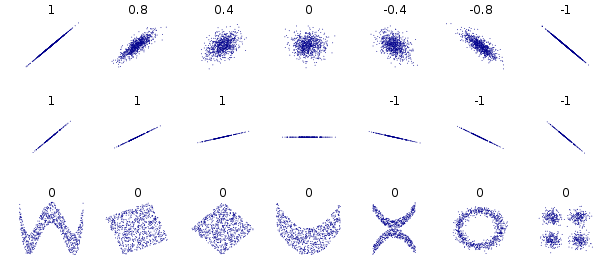
\includegraphics[width = 0.8\textwidth]{./figures/wiki_corr_example.png}
  \caption{Plotted are scatter points of
  $(x,y)$ pairs, with their empirical correlations
  (Exercise~\ref{ex:sample_corr}). Correlation measures the linear relationship
  between two random variables; however, zero correlation
  does not rule out other, nonlinear relationships.
  Figure taken from \url{https://en.wikipedia.org/wiki/Correlation}.}
  \label{fig:wiki_corr}
\end{figure}

\begin{exercise}[Best linear predictor]
As in Exercise~\ref{ex:predictions},
suppose data comes in pairs $(X, Y)$.
In the previous exercise, we saw that
the best predictor $g(X)$ was the conditional
expectation $\E(Y | X)$.

Here, we restrict ourselves to letting $g$
be a linear function, that is, predictors of the form
\begin{align*}
  g(X) = \beta X + \gamma
\end{align*}
for $\beta, \gamma\in\mathbb{R}$.

We again want to minimize the MSE \eqref{eq:mse}.

\begin{enumerate}[label = (\alph*)]
  \item Show that for fixed $\beta$,
  the unique $\gamma$ which minimizes the MSE
  if $\gamma^*(\beta) = \E(Y) - \beta \E(X)$.
  \item Now plug in $\gamma = \gamma^*(\beta)$,
  and show that the optimal $\beta$ is
  $\beta^*=\cov(X, Y) / \var(X)$.
  \item Apply the plug in principle by
  computing the
  variance/covariance under the empirical distribution,
  and find
  the sample formula for the best linear predictor.
  (In contrast, the solutions in (a) and (b) are
  \textit{population} formulas). 
\end{enumerate}

\end{exercise}

\end{document}
